\section{C-Line Mechanism: Trusted-Action Selection}

The C-line began as a policy-regularization track. Initial smoke experiments showed that plain TD3+BC was a weak anchor on \texttt{hopper-medium-replay-v2}, while ReBRAC-lite and SSAR were stronger. This raised a mechanism question: is SSAR stronger because it regularizes more, or because it regularizes toward better-selected actions?

Our evidence points to trusted-action selection. A cheap SSAR variant without IQL-based trusted selection performs much worse than full SSAR. Naive substitutes, including return-ranked trust, online Q-gap trust, and behavior-consistency trust, do not reliably solve the problem. This suggests that the useful signal is not arbitrary weighting; it is the choice of which dataset actions deserve trust.

ATLAS tests whether this trusted-action signal can be distilled. Given a cached SSAR/IQL-qv teacher, ATLAS trains a selector
\[
g_\phi(s,a) \in [0,1],
\]
which maps a state-action pair to a trust score. This score is then used as a weight in TD3+BC-style learning.

In the current implementation plan, $g_\phi$ is a small multilayer perceptron over the concatenated state-action vector, trained with binary cross entropy on teacher-derived trusted-action labels. The selector is not an actor or critic replacement; it only controls how strongly the actor is regularized toward each dataset action.

\[
\mathcal{L}_{\mathrm{actor}}
= \mathcal{L}_{Q}
+ \lambda(t)\,\mathbb{E}_{(s_i,a_i)\sim\mathcal{D}}
\left[
  w_i \lVert \pi_\theta(s_i) - a_i \rVert_2^2
\right],
\qquad
w_i = \mathrm{stopgrad}(\mathrm{clip}(g_\phi(s_i,a_i),0,1)).
\]

For offline training, $\lambda(t)$ is fixed. For online fine-tuning, the first diagnostic test is whether this regularization should stay fixed or follow a linear release schedule:
\[
\lambda(t) = \lambda_0 \max(0, 1 - t/K).
\]
This release schedule is intentionally simple. The P0 panel shows that it is not sufficient: it reduces some over-constraint but does not make ATLAS or SSAR/IQL-qv teacher labels beat the TD3+BC final online score. We therefore treat release as a diagnostic baseline, not as the final method.

\todobox{C-line owner: add cost/time numbers: SSAR full IQL-qv preselection vs ATLAS post-cache selector training.}

After the P0 panel exposed constraint trapping, we added one small online diagnostic: Q-filtered trust. During online fine-tuning, the teacher BC weight is multiplied by
\[
m_i = \sigma\left(\frac{Q_\psi(s_i,a_i) - Q_\psi(s_i,\pi_\theta(s_i))}{\tau}\right),
\qquad
\tilde{w}_i = w_i \left(m_{\min} + (1-m_{\min})m_i\right).
\]
This keeps a teacher-labeled dataset action only when the current critic still rates it above the actor action. It is intentionally a diagnostic gate, not a fully validated algorithm.

The current claim is intentionally limited. ATLAS is not presented as a new SOTA offline RL algorithm or as a solved online fine-tuning method. It is a mechanism probe showing that aligned teacher trust labels matter for offline initialization and can be reused after the expensive teacher cache has been produced.

\begin{figure}[t]
\centering
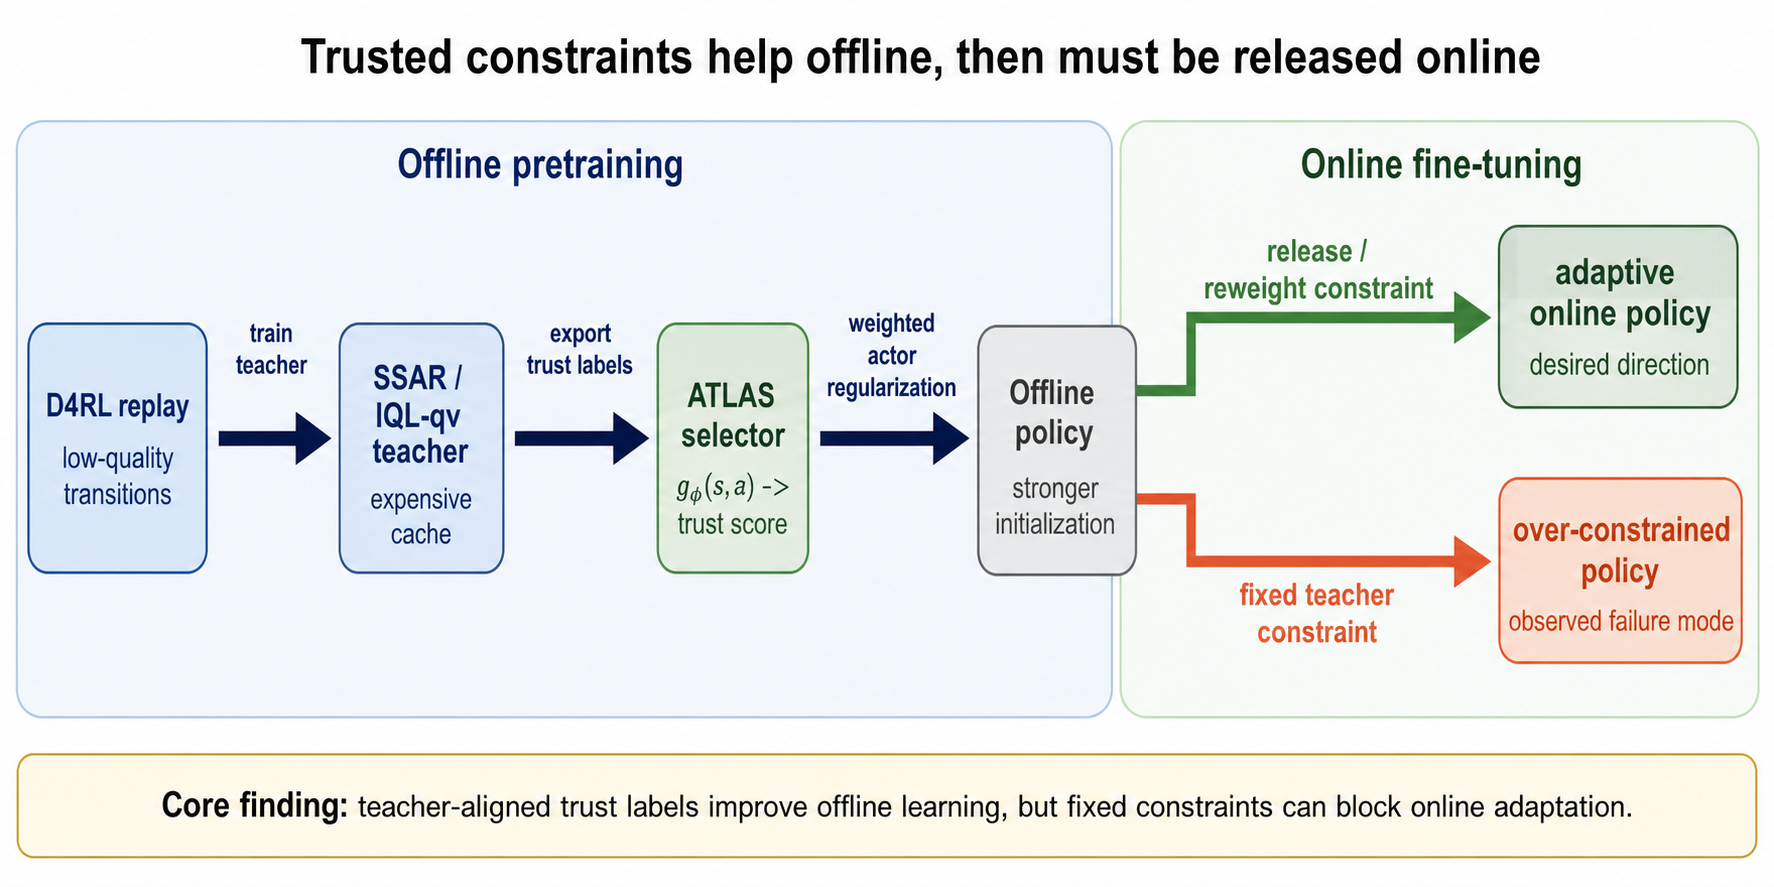
\includegraphics[width=\linewidth]{../figures/fig2_trusted_constraint_transfer_image2.png}
\caption{Trusted-constraint transfer. ATLAS distills trusted-action labels from a cached SSAR/IQL-qv teacher for offline learning, while the online phase exposes the need to release or reweight the constraint.}
\label{fig:atlas-mechanism}
\end{figure}
